\chapter[Paleomagnetism of the southwestern Laurentia large igneous province and Cardenas Basalt: pulsed magmatism during rapid late Mesoproterozoic plate motion][southwestern Laurentia large igneous province]{Paleomagnetism of the southwestern Laurentia large igneous province and Cardenas Basalt: pulsed magmatism during rapid late Mesoproterozoic plate motion}

\let\thefootnote\relax\footnote{Zhang, Y., Anderson, N., Mohr, M.T., Schmitz, M.D., Macdonald, F.A., Nelson, L.L., Thurston, O.G. Guenthner, W.R., Karlstrom, K.E., Swanson-Hysell, N.L. (2024). Paleomagnetism of the southwestern Laurentia large igneous province and Cardenas Basalt: pulsed magmatism during rapid late Mesoproterozoic plate motion. Submitted to JGR: Solid Earth.}

\section{Abstract}

Mafic intrusions, lava flows, and felsic plutons in southwestern Laurentia have been hypothesized to be associated with the emplacement of a late Mesoproterozoic large igneous province. Improved geochronologic data resolve distinct episodes of mafic magmatism in the region. The ca. 1098 main pulse of southwestern Laurentia large igneous province (SWLLIP) magmatism is recorded by mafic intrusions across eastern California to central Arizona. A younger episode of volcanism resulted in eruptions that formed the ca. 1082 Ma Cardenas Basalt---the uppermost unit of the Unkar Group in the Grand Canyon. Using the interpretation that the mafic intrusions within the Unkar Group were feeders to the lavas, a paleomagnetic pole was developed by combining data from the intrusions and the lavas. With the updated geochronological constraints, we develop new paleomagnetic data from mafic sills in the SWLLIP. Overlapping poles between the Death Valley sills and rocks of similar age in the Midcontinent Rift is inconsistent with large-scale Cenozoic vertical axis rotations in Death Valley. We also develop a new paleomagnetic pole from the ca. 1082 Ma Cardenas Basalt (pole longitude=183.9\textdegree E, pole latitude=15.9\textdegree N, A$_{95}$=7.4\textdegree, N=18). The new paleomagnetic data are consistent with the pole path developed from time-equivalent rocks of the Midcontinent Rift, supporting interpretations that changing pole positions are the result of rapid equatorward motion. These data add to the record of Laurentia's rapid motion from ca. 1110 to 1080 Ma that culminated in collisional Grenvillian orogenesis and the assembly of Rodinia. 

\section{Introduction}

The ancient North American craton (Laurentia) has a rich record of Stenian (late Mesoproterozoic) mafic magmatism. In the Midcontinent Rift of the Lake Superior region, punctuated episodes of voluminous intrusions and associated volcanism have been dated between 1109-1084 Ma with high-precision geochronology (Figure \ref{fig:SWLLIP_overview}). Paleomagnetic data from these well-preserved and well-dated rift-related rocks within the Midcontinent Rift make up the majority of the Stenian database of paleomagnetic poles for Laurentia \citep{Evans2021a}. These data provide central constraints on global paleogeography during the assembly of supercontinent Rodinia \citep{Swanson-Hysell2021c, Evans2021b}. 

In southwestern Laurentia, widespread Stenian magmatism led to the emplacement of mafic intrusions and lava flows as well as felsic plutons (Figure \ref{fig:SWLLIP_overview}A; \cite{Wrucke1966a, Shride1967a, Hendricks1972a, Howard1991a, Bright2014a}). Based on petrologic and geochemical data \cite[e.g.][]{Wrucke1966a, Wrucke1972a, Hammond1986a}, it was previously suggested that the mafic intrusions in the region were contemporaneous. However, in comparison to the Midcontinent Rift where extensive high-precision zircon U-Pb geochronology data have been developed (typically with analytical uncertainties $<$1 Myr; \cite[e.g.][]{Swanson-Hysell2019a}), most ages from rocks associated with the Stenian southwestern Laurentia magmatism have been relatively imprecise (e.g. as compiled and developed in \cite{Bright2014a}). The broadly overlapping ages, albeit with large uncertainties, of rocks that outcrop in California, Arizona, New Mexico, and Mexico led \cite{Bright2014a} to hypothesize that they could be grouped as the southwestern Laurentia large igneous province (SWLLIP). \cite{Bright2014a} further suggested that a temporal overlap of magmatism in the SWLLIP and in the Midcontinent Rift was the result of a geodynamic linkage. However, the available geochronology data from the SWLLIP at the time was not precise enough to test this relationship with the distinct magmatic intervals within the Midcontinent Rift. 

\begin{figure}[h!]
\centering
\includegraphics[width=0.75\textwidth]{figure/Zhang2024b/overview.pdf}
\caption{ (A) Map of North America showing the inferred extent of the southwestern Laurentia large igneous province (SWLLIP) modified from \cite{Bright2014a} in light brown color, a more strict version of the inferred extent of the SWLLIP based on encircling sills dated to be ca. 1098 Ma through the high-precision geochronology data of \cite{Mohr2024a} in dark brown, together with the Pikes Peak batholith \citep{Green1992b}, and the inferred extent of the Midcontinent Rift. The inferred trace of the Grenville Front is modified from \cite{Rivers2015a}. The inset boxes show the extent of maps in Figure \ref{fig:geologic_maps}. (B) Summary of high-precision zircon U-Pb geochronology data from southwestern Laurentia \citep{Mohr2024a} and from the Midcontinent Rift, highlighting the Duluth Complex and the associated North Shore Volcanic Group \citep{Swanson-Hysell2019a, Swanson-Hysell2021a}, the Michipicoten Island Formation \citep{Fairchild2017a}. The 1082.6 $\pm$ 0.3 Ma Colorado River Trough sill is located in the Dead Mountains in southeastern California. Each black bar represents a $^{206}$Pb/$^{238}$U zircon weighted mean age. The colored shaded regions associated with the black bars represent uncertainties of the mean ages at 95\% confidence level calculated with a Student's-T multiplier.}
\label{fig:SWLLIP_overview}
\end{figure}
    
Due to sparse geochronology data, temporal relationships between units in southwestern Laurentia are mostly inferred. In the Grand Canyon, it has been hypothesized that thick mafic sills and dikes that intrude Unkar Group sedimentary rocks are feeder systems for the Cardenas Basalt lava flows which are the uppermost unit of the Unkar Group \cite[e.g.][]{Hammond1990a, Timmons2005a}. This hypothesis is based on the spatial proximity and trace and major element concentration similarities of lava flows and nearby intrusions \citep{Larson1994a}. No direct field evidence exists for feeder relations. \cite{Hendricks1989a} considered the sills and flows to be from the same parent magma, but did discuss a possible interpretation that the more differentiated flows erupted later than the emplacement of the sills. Applying the assumption that the extrusive and intrusive rocks were coeval, \cite{Weil2003a} developed a paleomagnetic pole by grouping data derived from thirteen mafic intrusions and three Cardenas Basalt lava flows in the Grand Canyon. Similar directions had previously been developed for two Cardenas lava flows by \cite{Elston1973a}. \cite{Weil2003a} assigned an age of 1090.6 $\pm$ 4.5 Ma (2$\sigma$) to their pole based on an $^{40}$Ar-$^{39}$Ar age they developed from biotite interpreted to have formed within the host Unkar sedimentary rocks during the intrusion of a mafic sill. 

Paleomagnetic data have also been developed from SWLLIP mafic sills that intrude Apache Group sedimentary rocks in central Arizona \citep{Helsley1972a, Donadini2011a}. These studies interpreted sills with normal-polarity paleomagnetic directional data as coeval. \cite{Donadini2011a} developed a mean pole from some normal-polarity sills and considered the age of the pole to be that of a baddeleyite U-Pb age of 1088 $\pm$ 11 Ma (2$\sigma$; age from one sill later published by \cite{Bright2014a}). Although \cite{Harlan1993a} also obtained paleomagnetic samples of mafic sills in the same region with clearer distinction between individual cooling units, that the normal paleomagnetic pole of \cite{Donadini2011a} was reported with paired radiometric age assignment led it to be the pole that is included in recent curated paleogeographic compilations \cite[e.g.][]{Evans2021a}. Other sills in the region record reversed directions with steeper inclinations relative to the normal polarity directions \citep{Harlan1993a, Donadini2011a}. In the field guide of \cite{Donadini2012a}, an age of 1119 $\pm$ 10 Ma (weighted mean of $^{207}$Pb/$^{206}$Pb date of 2 baddeleyite grains) and a age of 1111.6 $\pm$ 8.9 Ma (concordia intercept age of a combination of baddeleyite and zircon dates) were reported for sills of reversed polarity---these geochronology data remain unpublished. Both the steep reversed directions and the geochronological data are consistent with these sills being emplaced during an interval of reversed polarity prior to or during ca. 1109 to 1105 Ma early-stage Midcontinent Rift magmatism \citep{Vervoort2007a, Swanson-Hysell2019a}.

More recently, \cite{Mohr2024a} developed chemical abrasion-isotope dilution-thermal ionization mass spectrometry (CA-ID-TIMS) high-precison U-Pb geochronology data from zircon separated from differentiated zones in thick mafic sills in southwestern Laurentia and from zircon separated by bulk dissolution methods (applying the approach of \cite{Oliveira2022a}) from a thick lava flow within the Cardenas Basalt (Figure \ref{fig:cardenas_strat}). Three sills in Death Valley were dated at 1097.91 $\pm$ 0.29 Ma, 1098.27 $\pm$ 0.27 Ma, and 1098.09 $\pm$ 0.91 Ma, two sills in western Grand Canyon at 1098.16 $\pm$ 0.59 and 1098.09 $\pm$ 0.34 Ma, and one sill in central Arizona at 1097.97 $\pm$ 0.12 Ma (all ages are presented with analytical uncertainties at 95\% confidence which is calculated including a Student’s-T multiplier; \cite{Mohr2024a}). These ages agree with each other within uncertainty (Figure \ref{fig:SWLLIP_overview}B) and suggest that the mafic intrusions across the region were rapidly emplaced in $\sim$0.25 Myr \citep{Mohr2024a}. The data indicate an episode of LIP-style mafic magmatism ca. 1098 Ma in southwestern Laurentia that postdates the early plateau stage of volcanism in the Midcontinent Rift and predates the emplacement of the ca. 1096 Ma Duluth Complex and thick main stage rift volcanics (Fig. \ref{fig:SWLLIP_overview}). The data are consistent with a model where a plume head arrived ca. 1098 Ma under southwestern Laurentia leading to generation of melt and the emplacement of thick mafic intrusions. This plume could have then spread along the base of the lithosphere toward the Midcontinent Rift where it facilitated the reinvigoration of magmatism associated with the emplacement of the Duluth Complex and the North Shore Volcanic Group \citep{Mohr2024a}. In addition, \cite{Mohr2024a} developed a new zircon U-Pb age of 1082.18 $\pm$ 1.25 Ma (95\% confidence) from a Cardenas Basalt lava flow. That age indicates that the eruption of the lavas postdated the widespread ca. 1098 Ma mafic intrusions by $\sim$16 Myr (Figure \ref{fig:SWLLIP_overview}B). Given the rapid apparent polar wander shown by the ca. 1109-1080 Ma Keweenawan Track \citep{Swanson-Hysell2019a}, the $\sim$16 Myr age difference between the Cardenas Basalt and thick mafic sills predict that they should record distinct paleomagnetic pole positions separated by a large angular distance. With the new chronological insights in hand, we develop new paleomagnetic data from the dated mafic sills and additional undated Mesoproterozoic intrusions in Death Valley and the Grand Canyon. We also develop new paleomagnetic data from lava flows of the Cardenas Basalt within the Grand Canyon with an increased number of sites as well as volcanostratigraphic context. 

\section*{Geological Background}
\subsection*{Mafic intrusions in the Crystal Spring Formation, Death Valley}

Rocks in the Death Valley region record the geological evolution of the southwestern margin of Laurentia since ca. 1.8 Ga in the Paleoproterozoic Era (\cite{Tapani-Ramo1998a}; Figure \ref{fig:geologic_maps}A, \ref{fig:DV_GC_strat_columns}). The basement rocks include Paleoproterozoic para- and orthogneiss \citep{Wasserburg1959a, Barth2000a, Strickland2013a} and early Mesoproterozoic porphyritic quartz monzonite \citep{Labotka1980a}. The Pahrump Group is a 1.5 to 4 km thick mixed carbonate and siliciclastic succession that unconformably overlies these basement lithologies (Figure \ref{fig:DV_GC_strat_columns}; \cite{Wright1974a, Macdonald2013a}. Formations of the Pahrump Group include the Mesoproterozoic Crystal Spring Formation, the Tonian Horse Thief Springs Formation, the Tonian Beck Spring Dolomite, and the Cryogenian Kingston Peak Formation \citep{Macdonald2013a, Mahon2014a}. A $>$300 Myr unconformity separates the Crystal Spring Formation, which contains mafic sills, and the overlying Horse Thief Springs Formation, which contains $<$775.4 $\pm$ 0.7 Ma detrital zircon (\citep{Mahon2014a, Dehler2023a}; Figure \ref{fig:DV_GC_strat_columns}) and does not contain the sills. The region experienced Permian-Triassic contraction and magmatism \citep{Snow1991a, Stevens1997a} followed by the Mesozoic Cordilleran orogeny \citep{Burchfiel1992a, Burchfiel1970a, Snow1991a}. Neogene felsic and mafic magmatism (Figure \ref{fig:geologic_maps}), high-angle normal faults, basement detachment faults, as well as transform faults associated with extensional tectonism are widespread in the region \citep{Wright1974a, Snow2000a, Calzia2000a, Wrucke2007a, Renik2013a}. 

\begin{figure}[h!]
\centering
\includegraphics[width=0.85\textwidth]{figure/Zhang2024b/geologic_maps.png}
\caption{\footnotesize (A) Simplified geologic map of southern Death Valley, CA, (with units modified from \cite{Workman2003a} and \cite{Wrucke2007a}) showing the location of mafic sills that were sampled for paleomagnetism in this study and geochronology in \cite{Mohr2024a}. The Mesozoic and Cenozoic intrusions that occur in close proximity to the sills have the potential to have resulted in variable degrees of alteration and magnetic overprints. The sills typically were emplaced parallel to host sedimentary beds in the Crystal Spring Formation, but also intrude older crystalline lithologies. In the field, we collected multiple orientation measurements for sills from contact planes or adjacent sedimentary beds. An average orientation was calculated for each sill and was used to tilt-correct the paleomagnetic data. The representative orientations summarized on the map show that different regions are variably tilted. (B) Simplified geologic map of the Grand Canyon with units modified from \cite{Billingsley2000a} and \cite{Billingsley2003a} showing sedimentary rocks of the Unkar Group, mafic sills and dikes that intruded the sedimentary rocks, and the Cardenas Basalt that is the uppermost unit within the Unkar Group (Fig. \ref{fig:DV_GC_strat_columns}) `RM' stands for river mile using the widely adopted nomenclature of tracking distance through Grand Canyon. Bedding orientations at Nankoweap Canyon were collected from lava flow tops and the bedding of the overlying Nankoweap Formation which have very similar orientations; orientations at Lava Chuar Canyon were collected from the lava flow tops; orientations at Basalt Canyon were collected from lava flow tops, interflow sedimentary rocks, and the Dox Formation stratigraphically below the Cardenas Basalt. These bedding measurements were used for tilt-correcting paleomagnetic data. All geochronology data shown are U-Pb zircon ages from \cite{Mohr2024a}.}
\label{fig:geologic_maps}
\end{figure}

Tilting of crustal blocks related to Neogene extension in Death Valley resulted in the exposure of numerous sills and dikes that intrude the basement rocks and the Crystal Spring Formation. The thickness of the mafic sills ranges from $<$1 meter to over a hundred meters \citep{Wright1968a, Hammond1983a}. Chilled margins with the Crystal Spring Formation have a finer grain size than the interiors. Olivine, pyroxene and plagioclase are typically altered within the sills \citep{Hammond1983a}. Based on petrological analyses, \cite{Hammond1983a} interpreted that the alteration dominantly happened during mafic emplacement. Talc deposits up to 30 m thick are developed along contacts between the mafic and the dolomitic lithofacies of the Crystal Spring Formation \citep{Wright1968a}. Mining of talc within these contact metamorphosed zones has resulted in striking white scars in the regional landscape next to some of the sills.

\cite{Heaman1992b} developed U-Pb TIMS dates from baddeleyite separated from pegmatitic zones within two mafic sills that outcrop in the southern Ibex Hills near Saratoga Spring in Death Valley National Park and in the Kingston Range (Figure \ref{fig:geologic_maps}A). Due to Pb loss in baddeleyite, the resultant dates are discordant, with interpreted concordia upper intercept ages of 1069 $\pm$ 3 Ma and 1087 $\pm$ 3 Ma (2$\sigma$). The sill from Saratoga Spring yielded a lower intercept age of ca. 65 Ma which \cite{Heaman1992b} interpreted to be related to growths of younger zircon rims around older baddeleyite crystals. In addition, \cite{Wasserburg1964a} obtained a ca. 235 Ma K-Ar age from a Mesoproterozoic mafic sill in the Crystal Spring Formation that outcrops in Warm Spring Canyon. Although the baddeleyite lower intercept age and the K-Ar age are roughly constrained, these ages are consistent with the mafic sills having been affected by Mesozoic and Cenozoic metamorphism \citep{Snow1989a, Snow2000a}. Recently, \cite{Mohr2024a} extracted zircons from granophyric segregations within two mafic sills from Warm Spring Canyon and one from the central Ibex Range (Figure \ref{fig:geologic_maps}A). High-precision CA-ID-TIMS zircon U-Pb geochronology yielded indistinguishable $^{206}$Pb/$^{238}$U ages of 1097.91  $\pm$  0.29 Ma, 1098.27  $\pm$  0.27 Ma, and 1098.09  $\pm$  0.91 Ma from the three individual sills (95\% confidence; Figure \ref{fig:SWLLIP_overview}B, \ref{fig:geologic_maps}A, \ref{fig:DV_GC_strat_columns}). 

\begin{figure}[h!]
\centering
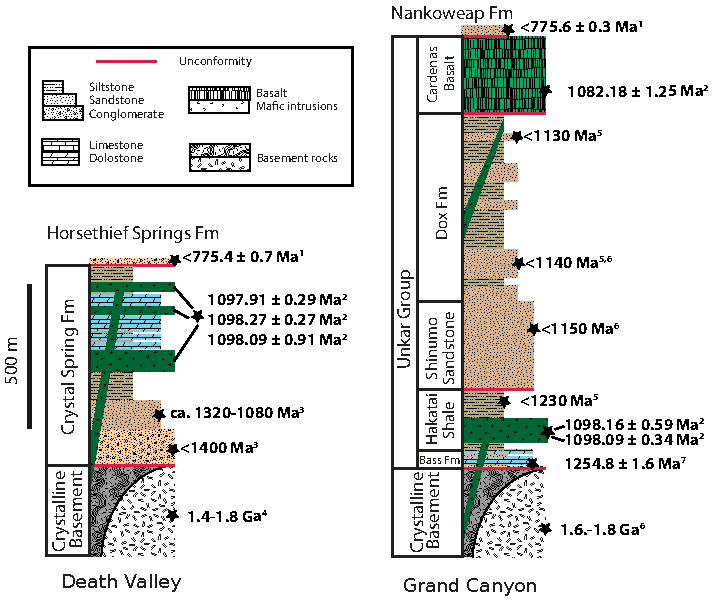
\includegraphics[width=\textwidth]{figure/Zhang2024b/DV_GC_Mesoproterozoic_strat_columns.pdf}
\caption{\footnotesize Simplified regional Mesoproterozoic stratigraphy in context of older basement rocks and younger Neoproterozoic sedimentary rocks and compiled geochronology in Death Valley and Grand Canyon. Red lines are unconformities. Black stars are existing radioisotopic age constraints. $^1$ CA-ID-TIMS U-Pb detrital zircon dates \citep{Dehler2023a}; $^2$ CA-ID-TIMS U-Pb zircon dates \citep{Mohr2024a}; $^3$ LA-MC-ICPMS U-Pb detrital zircon dates \citep{Mahon2014b}; $^4$ muscovite, biotite, and potassium feldspar $^{40}$K-$^{40}$Ar and $^{87}$Rb-$^{87}$Sr dates \citep{Lanphere1964b}, biotite, muscovite, and hornblende$^{40}$Ar-$^{39}$Ar dates \cite{Labotka1985a}, and SHRIMP U-Pb zircon and monazite dates \cite{Barth2001a, Barth2009a}; $^5$ \cite{Mulder2017a}; $^6$ detrital zircon and detrital muscovite dates \cite{Timmons2005a}; $^7$ TIMS U-Pb zircon dates from an ash layer \cite{Timmons2005a}.}
\label{fig:DV_GC_strat_columns}
\end{figure}

\subsection*{Mafic intrusions in the Unkar Group}

The Grand Canyon Supergroup is divided into the Mesoproterozoic Unkar Group and the Neoproterozoic Chuar Group \citep{Gundy1951a, Elston1989a, Dehler2017a}. The $\sim$2 km-thick Unkar Group contains the Bass Formation, Hakatai Shale, Shinumo Quartzite, Dox Formation, and Cardenas Basalt (Figure \ref{fig:DV_GC_strat_columns}; \cite{Beus1974a, Elston1989a}). It is interpreted that the Unkar Group dominantly records shallow marine and fluvial depositional environments \citep{Elston1989a, Sears1990a, Hendricks1989a, Timmons2005a}. Siliclastic deposition continued during eruption of the Cardenas Basalt resulting in interflow siltstone and sandstones---often with mudcracks and current ripples respectively  (Fig. \ref{fig:cardenas_strat}). Unkar Group strata typically dip at $\sim$10\textdegree\ to the northeast (Figure \ref{fig:geologic_maps}) toward normal faults that dip $\sim$60\textdegree\ to the southwest \citep{Sears1973a, Timmons2012a}. Intraformational faults and large thickness changes in sedimentary units across faults indicate that the Unkar Group was deposited in an extensional tectonic setting \citep{Sears1990a, Karlstrom1998a, Timmons2001a}. 

Numerous mafic sills and dikes intrude the Unkar Group, but not the overlying Chuar Group (Figures \ref{fig:geologic_maps}B and \ref{fig:DV_GC_strat_columns}; \cite{Elston1989a}). Sills typically intrude the Bass Formation and the Hakatai Shale of the lower Unkar Group \citep{Hendricks1989a} whereas mafic dikes have been mapped to crosscut the Shinumo Sandstone and the Dox Formation of the upper Unkar Group \citep{Timmons2012a}. Typical dike plane orientations are subparallel to NW-trending faults in the Unkar Group \citep{Huntoon1996a, Timmons2012a}. The sills typically range in thickness between 20 to over 100 meters and are alkali-olivine basalt in composition (\cite{Hendricks1989a, Larson1994a}; Figure S1). Given their spatial proximity and stratigraphic relationship, it had been commonly inferred that all mafic intrusions in the Unkar Group are feeders to the Cardenas Basalt \cite[e.g.][]{Huntoon1996a, Timmons2012a}, though no direct feeder relationships have been observed.

The interior of the thick mafic sills are medium- to coarse-grained with subophitic to ophitic texture characterized by plagioclase and olivine grains being enclosed by poikilitic pyroxenes \citep{Hendricks1989a}. The intrusions are fine-grained at their margins where they are chilled against the Unkar sedimentary rocks.  Some of the sill interiors contain zircon-bearing segregations \citep{Mohr2024a}, which were dated with high-precision CA-ID-TIMS $^{206}$Pb/$^{238}$U at 1098.16 $\pm$ 0.59 Ma at Hotauta Canyon (river mile [RM] 107) and 1098.09 $\pm$ 0.34 Ma at Stone Creek (RM 132) (Figure \ref{fig:SWLLIP_overview}B, \ref{fig:geologic_maps}B; 2$\sigma$ uncertainties). 

\subsection*{Cardenas Basalt}

The Cardenas Basalt at the top of the Unkar Group exclusively outcrops in eastern Grand Canyon (Figure \ref{fig:geologic_maps}). The most complete section of the Cardenas Basalt outcrops at the Basalt Canyon area where $\sim$315 meters of lava flows and associated interflow sedimentary rocks are preserved up to the unconformity between the volcanics and the overlying Nankoweap Formation (Figure \ref{fig:geologic_maps}B, \ref{fig:cardenas_strat}; \cite{Lucchitta1983a, Hendricks1989a}). Cardenas Basalt also outcrops with variable thicknesses at localities including Lava Chuar Canyon and Nankoweap Canyon (Figure \ref{fig:geologic_maps}B, \ref{fig:cardenas_strat}). The lava flows are typically trachy-basaltic andesite in composition, overall having higher SiO$_2$ values than the mafic intrusions in the Unkar Group (Figure S1; \cite{Hendricks1989a, Larson1994a}).

\begin{figure}[h!]
\centering
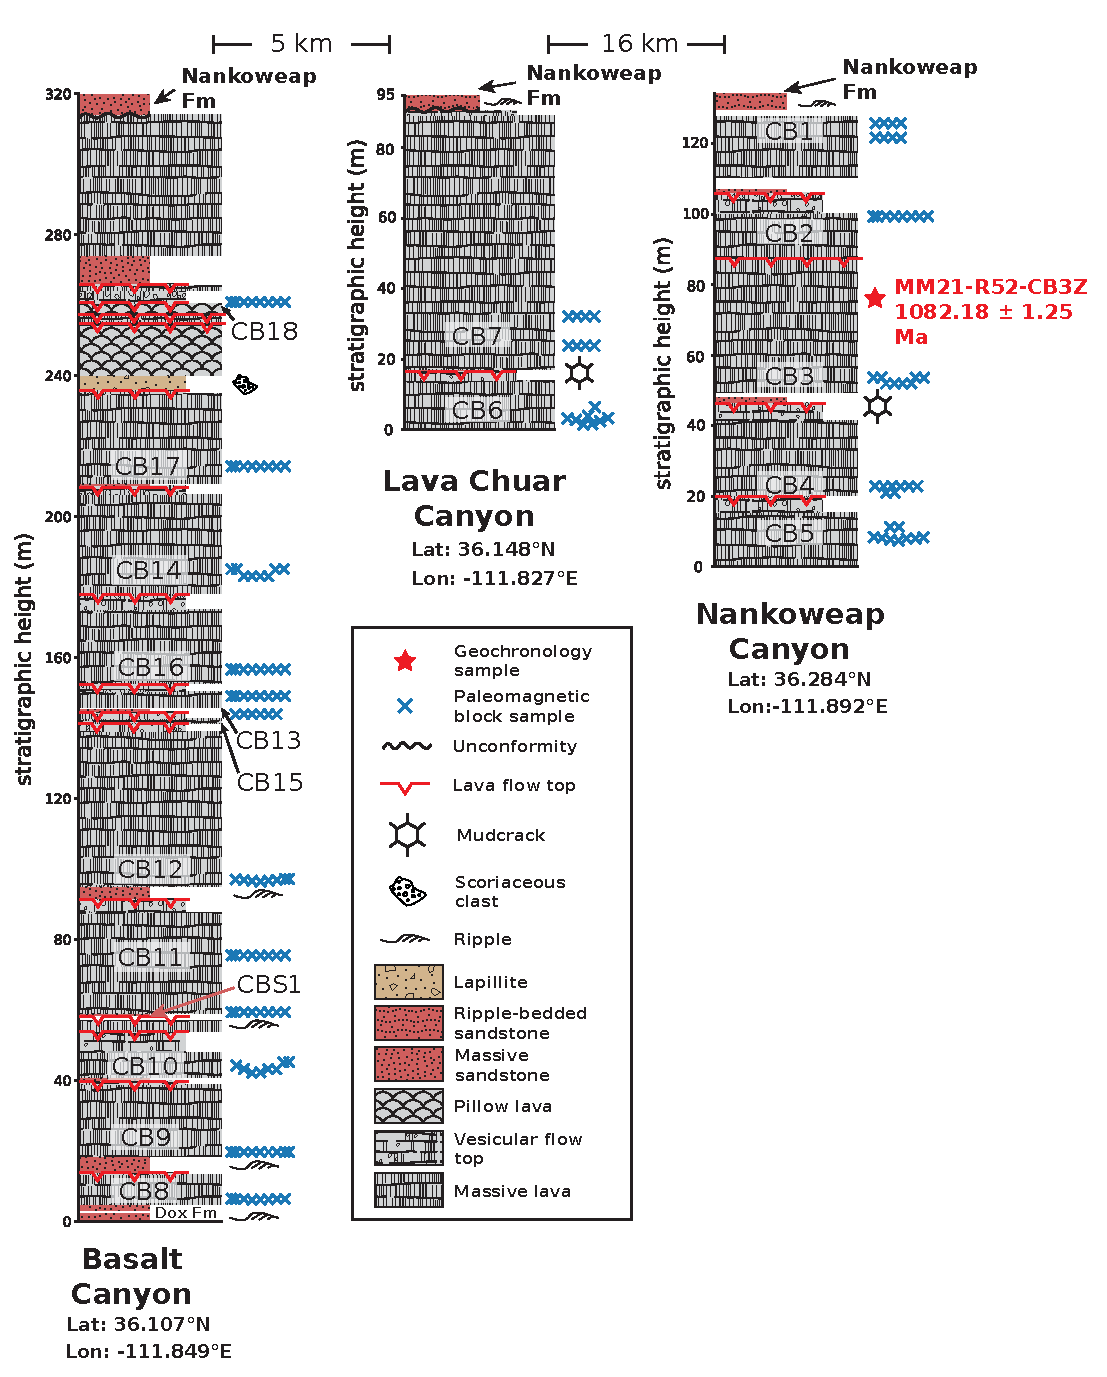
\includegraphics[width=0.82\textwidth]{figure/Zhang2024b/Cardenas_strat_uniform_scale.pdf}
\caption{Volcanostratigraphy of the Cardenas Basalt at Basalt Canyon, Lava Chuar Canyon, and Nankoweap Canyon measured in this study. Section locations are shown in Figure \ref{fig:geologic_maps}B. Stratigraphic locations of the collected paleomagnetic samples and the geochronology sample dated by \cite{Mohr2024a} are shown. The interflow sandstones and vesicular lava flow tops distinguish individual lava flows such that paleomagnetic samples from each lava flow constitute a site (labeled as `CB' with distinct numbers). The latitude and longitude values correspond to the base of the stratigraphic sections.}
\label{fig:cardenas_strat}
\end{figure}

Previous studies constructed volcanostratigraphic sections of the Cardenas Basalt at Basalt Cliffs, Ochoa Point, Basalt Canyon, and Lava Chuar Canyon \citep{Lucchitta1983a, Hendricks1989a}. In particular, \cite{Hendricks1989a} developed a stratigraphic section at Basalt Canyon with detailed petrologic and lithologic descriptions. In this study, we investigated three sections at Basalt Canyon, Lava Chuar Canyon, and Nankoweap Canyon (Figure \ref{fig:geologic_maps}). We measured volcanostratigraphic sections with a particular focus on determining individual lava flows that represent distinct cooling units such that paleomagnetic samples collected from a single lava flow are considered to capture the same snapshot of the geomagnetic field as they cooled (i.e. a paleomagnetic site; Fig. \ref{fig:cardenas_strat}). Flow boundaries can be delineated by progressive changes in vesiculation and by highly vesiculated flow tops and/or interflow clastic sedimentary rocks (Figure \ref{fig:cardenas_strat}, \ref{fig:field_photo}E). Interflow sedimentary rocks between lava flows are common (Figure \ref{fig:cardenas_strat}).

At Basalt Canyon, flows in the initial 95 meters are subophitic to ophitic in texture and heavily weathered with a greenish color (Figure \ref{fig:field_photo}B). These flows form slopes characterized by small weathered basalt fragments that often are dislodged pyroxene oikocrysts. Walking on steep slopes mantled by these oikocrysts is like walking on ball bearings. \cite{Walcott1883a} and \cite{Lucchitta1979a} noted that those flows experienced spilitic alteration, interpreted as the result of subaqueous eruptions in a tidal flat or deltaic environment. The claim has also been made that there are pillows in these lower flows \citep{Stevenson1982a, Hendricks1974a}. However, our field observations, as well as those of \cite{Larson1994a} and \cite{Elston1976a}, did not find evidence of pillow lava indicative of subaqueous eruptions in these flows---note that spheroidal weathering can often be misidentified as pillows. While spheroidal weathering, granular grus piles, and ophitic textures on the weathered exposures are common, the features in these basal ophitic flows, including the presence of an observed pahoehoe flow top and basal pipe vesicles, are consistent with them being subaerially erupted sheet flows (Figure \ref{fig:field_photo}B). A ropy flow top consistent with pahoehoe lava flows was also reported in \cite{Hendricks1989a}. The upper 200 meters of Cardenas Basalt flows consist of more competent, cliff-forming lava flows that are finer-grained than the lower sequence. A 4-meter-thick volcaniclastic layer containing cobble- to boulder-sized scoriaceous volcanic clasts surrounded by tan-colored, fine-grained matrix occurs at stratigraphic height of $\sim$240 m (Figure \ref{fig:cardenas_strat}, \ref{fig:field_photo}D). \cite{Lucchitta1983a} named this unit the lapillite member of the Cardenas Basalt and interpreted that it likely formed as pyroclastic debris deposited by lahars. Pillow lavas typically 0.8 to 1 m wide with horizons of volcaniclastic materials consistent with subaqueous eruption are found near the top of the section, above the lapillite layer (Figure \ref{fig:field_photo}F). 

Shorter sections of Cardenas Basalt flows are exposed in Nankoweap Canyon (RM 52) and Lava Chuar Canyon (RM 65) (Figure \ref{fig:geologic_maps}B, \ref{fig:cardenas_strat}). Due to the less complete exposures at these two localities, the volcanostratigraphic correlations between the three localities cannot be unequivocally drawn. However, large lateral variability of individual lava flow thicknesses has been reported \citep{Lucchitta1983a}, indicating that lava flows likely pinch out laterally between the localities. Our stratigraphic sections at the three localities also show variable lava flow thicknesses directly below the Nankoweap Formation (Figure \ref{fig:cardenas_strat}) although this could reflect variability in erosional truncation. We treat the sampled lava flows sampled at different localities as distinct cooling units in this study with each being an individual paleomagnetic site (Figure \ref{fig:cardenas_strat}). The \cite{Mohr2024a} geochronology sample for the Cardenas Basalts comes from the interior of a 57 m thick lava flow at Nankoweap Canyon (Figure \ref{fig:field_photo}A; CB3). Four zircon microlites yielded a weighted mean $^{206}$Pb/$^{238}$U ages of 1082.18 $\pm$ 1.25 Ma (95\% confidence; Figure \ref{fig:SWLLIP_overview}B). 

\begin{figure}[h!]
\centering
\includegraphics[width=0.82\textwidth]{figure/Zhang2024b/field_photo.png}
\caption{Field photos of Cardenas Basalt. The site names correspond to those shown in the stratigraphic section in Figure \ref{fig:cardenas_strat}. (A) Coarse-grained interior of the 57 m thick CB3 lava flow at Nankoweap Canyon from which zircon were extracted and dated by \cite{Mohr2024a}. (B) Ophitic texture in the interior of flow CB9 at Basalt Canyon. Individual oikocrysts reach diameters of 9 mm. (C) Contact between two individual lava flows CB14 and CB16 (meter level 178 in Fig. \ref{fig:cardenas_strat}) The massive flow bottom of the upper flow is more resistant to weathering than the recessive vesiculated flow top of the underlying flow. (D) The volcaniclastic marker bed containing scoriaceous volcanic clasts surrounded by tan-colored, very fine-grained matrix at 236 to 240 m in the Basalt Canyon section. (E) Amygdaloidal flow top of CB16. Elongate amygdules indicate that vesicles were stretched during flow. (F) Pillow lavas near the top of the exposed stratigraphy at Basalt Canyon (within interval from meter level 240 to 257; Fig. \ref{fig:cardenas_strat}). }
\label{fig:field_photo}
\end{figure}

\section*{Methods}

A total of 123 samples from 15 individual mafic sills were collected from the Death Valley region (Fig. \ref{fig:geologic_maps}A). Core samples were collected with a gasoline-powered drill outside of Death Valley National Park and block samples were collected from sills inside the park. In the Grand Canyon, a total of 184 block samples were collected from 18 individual Cardenas Basalt lava flows, 1 baked interflow sedimentary bed, and 5 mafic intrusions within the Unkar Group. When sampling the intrusions, we preferentially targeted the finer-grained margins of flows and intrusions over the coarser-grained interiors. Typically, 6-9 samples were collected at each site. Both magnetic compass and sun compass were used when orienting the drill cores and block samples in the field. Sun compass orientations were preferentially used when available. In the lab, standard paleomagnetic cores were drilled from the block samples and then oriented relative to the oriented surfaces.

The locations of the paleomagnetic sites are shown in Figure \ref{fig:geologic_maps} and Table \ref{tab:pmag_data}, and the stratigraphic positions of block samples collected from the Cardenas Basalt are shown in Figure \ref{fig:cardenas_strat}. In western Grand Canyon, we sampled the 1098.16 $\pm$ 0.59 Ma sill in Hotauta Canyon as UI4 (RM 107) and the 1098.09 $\pm$ 0.34 Ma Stone Creek Canyon sill as UI5 (RM 132). In the eastern canyon, we sampled the Hance dike north to the Hance Rapids (UI2; RM 77) and the Hance sill south to the rapids (UI3). Another undated mafic sill was sampled at Red Canyon (RM 77) which is south of the river at Hance Rapids along the tributary stream channel of Red Canyon (UI1; Figure \ref{fig:geologic_maps}B). In Death Valley, within Warm Spring Canyon, we sampled the 1097.91 $\pm$ 0.29 Ma sill as CS1 and the 1098.27 $\pm$ 0.27 Ma sill as CS4, and in Ibex Hills, we sampled the 1098.09 $\pm$ 0.91 Ma sill as CS7. Other undated sills are labeled in Figure (\ref{fig:geologic_maps}) and locations for all sites are available in the archived data repository (\url{https://zenodo.org/doi/10.5281/zenodo.10625967}). 

A suite of specimens from sills in the Crystal Spring Formation underwent step-wise thermal demagnetization up to 680 \textdegree C. An additional suite of sister specimens from some samples also underwent thermal demagnetization with an added step of a liquid nitrogen bath following the measurement of natural remanent magnetization. This demagnetization step can preferentially remove overprint magnetization held by multidomain titanomagnetite grains and potentially improve the resolution of the characteristic component. All specimens from the Cardenas Basalt and the mafic intrusions within the Unkar Group underwent step-wise thermal demagnetization up to 580 \textdegree C with some samples continuing up to 680 \textdegree C. The thermal demagnetization protocol had increasingly higher resolution approaching the Curie temperature of magnetite ($\sim$580\textdegree C) and N\'eel temperature of hematite ($\sim$680\textdegree C).

All demagnetization experiments were carried out in the magnetically shielded room at the UC Berkeley Paleomagnetism Lab. The typical magnetic field inside the shielded room is $<$500 nT. An ASC TD-48SC thermal demagnetizer with $<$10 nT field inside the chamber was used for the demagnetization steps. All remanence measurements were made on a 2G Enterprises DC-SQUID superconducting rock magnetometer. The PmagPy software package \citep{Tauxe2016a} was used to implement least-square fits \citep{Kirschvink1980a} to specimen demagnetization data. 

In the Death Valley region, multiple bedding orientations were measured along contacts between the sills and the host sedimentary rocks and along bedding of sedimentary rocks near the sills, and the averages of these measurements were used to tilt-correct paleomagnetic directions of each sill. In the Grand Canyon, the contact planes between the Hance sill and the adjacent sedimentary layers are poorly exposed. We collected bedding measurements from the nearby exposures of the Bass Formation for tilt correction. We also collected orientations from the Hance sill columnar joint planes---planes that are typically vertical prior to tilting. The best-fit plane orthogonal to the columnar joint planes has an orientation similar to the mean bedding plane of the Bass Formation. Bedding orientations of the host Hakatai Shale were used to tilt-correct the Hance dike paleomagnetic data. Bedding orientations were taken on the Cardenas Basalt flow tops and on interflow sediments for tilt correction. All bedding orientation data are available in the archived data repository (\url{https://zenodo.org/doi/10.5281/zenodo.10625967}).

\section*{Results and Interpretations}

Eight out of the 15 mafic sills from the Death Valley area yielded stable, consistent, and interpretable paleomagnetic directional data. All sites including 5 mafic sills, 18 lava flows, and 1 interflow sedimentary bed sampled in the Grand Canyon yielded well-grouped, consistent paleomagnetic directions. The site-level paleomagnetic statistics are summarized in Table \ref{tab:pmag_data}. Data to the individual measurement level are available in the MagIC database (private link for reviewer here: \url{https://earthref.org/MagIC/20009/d7aee057-ee64-4bb3-baa2-f69cb7852357}; \textit{this link will be updated to a doi upon acceptance}.).

\begin{sidewaystable}
\resizebox{0.95\textwidth}{!}{
\tiny
\begin{tabular}{p {1cm} p {2.5cm} p {1.5cm} p {2cm} p {2.3cm} p {0.5cm} p {1cm} p {1cm} p {1cm} p {1cm} p {1cm} p {1cm} p {1cm} p {1cm} }
\hline
site      & study region     & geologic type            & site latitude (\textdegree N) & site longitude (\textdegree E) & n  & dec$_{gc}$                    & inc$_{gc}$                   & dec$_{tc}$ & inc$_{tc}$ & k    & $\alpha_{95}$ (\textdegree) & vgp lat (\textdegree N) & vgp lon (\textdegree E) \\
\hline
CS1$^*$       & Death Valley & sill                 & 35.9688  & -116.9190 & 8  & 303.0                        &  50.0                        & 292.8   & 73.3    & 175  & 4.2  & 41.7     & 203.7    \\
CS2       & Death Valley & sill                 & 35.9651  & -116.9130 & 7  & 290.2                        & 43.2                        & 296.3   & 65.3    & 27   & 11.9 & 42.5     & 187.7    \\
CS6       & Death Valley & sill                 & 35.9618  & -116.8829 & 8  & 275.5                        & -4.7                        & 281.3   & 48.4    & 45   & 8.3  & 25.2     & 172.3    \\
CS7$^*$       & Death Valley & sill                 & 35.8154  & -116.3886 & 2  & 318.0                        & -8.0                        & 331.1   & 42.4    & 167  & 19.5 & 62.7     & 137.2    \\
CS8       & Death Valley & sill                 & 35.8114  & -116.3854 & 9  & 305.2                        & 5.2                         & 297.1   & 58.7    & 78   & 5.9  & 41.1     & 177.8    \\
CS9       & Death Valley & sill                 & 35.8112  & -116.3855 & 5  & 316.0                        & -2.0                        & 317.5   & 52.6    & 39   & 12.3 & 55.1     & 161.9    \\
CS12      & Death Valley & sill                 & 35.7789  & -116.1206 & 8  & 284.7                        & 2.3                         & 301.6   & 63.3    & 30   & 10.2 & 45.5     & 184.3    \\
CS13      & Death Valley & sill                 & 35.8187  & -116.0938 & 3  & 269.0                        & -13.7                       & 293.6   & 51.2    & 150  & 10.1 & 35.8     & 170.3    \\
CB1       & Grand Canyon & lava flow            & 36.2839  & -111.8919 & 8  & 249.3                        & 52.9                        & 270.3   & 51.1    & 200  & 3.9  & 18.4     & 184.5    \\
CB2       & Grand Canyon & lava flow            & 36.2836  & -111.8919 & 8  & 276.3                        & 56.5                        & 283.3   & 78.7    & 329  & 3.1  & 38.2     & 220.8    \\
CB3$^*$       & Grand Canyon & lava flow            & 36.2833  & -111.8928 & 7  & 261.3                        & 58.7                        & 249.3   & 52.9    & 56   & 8.1  & 5.1      & 196.5    \\
CB4       & Grand Canyon & lava flow            & 36.2831  & -111.8928 & 7  & 248.6                        & 35.0                        & 261.3   & 58.7    & 37.1 & 10.0 & 16.9     & 196.9    \\
CB5       & Grand Canyon & lava flow            & 36.2825  & -111.8914 & 9  & 241.6                        & 45.7                        & 276.3   & 56.5    & 71   & 6.2  & 25.3     & 186.8    \\
CB6       & Grand Canyon & lava flow            & 36.1458  & -111.8275 & 8  & 270.3                        & 51.1                        & 252.7   & 47.0    & 88   & 5.9  & 3.8      & 190.7    \\
CB7       & Grand Canyon & lava flow            & 36.1464  & -111.8269 & 8  & 283.3                        & 78.7                        & 269.9   & 42.5    & 106  & 5.4  & 14.1     & 178.5    \\
CB8       & Grand Canyon & lava flow            & 36.1072  & -111.8486 & 8  & 271.9                        & 53.0                        & 272.7   & 38.5    & 132  & 4.8  & 14.7     & 174.5    \\
CB9       & Grand Canyon & lava flow            & 36.1073  & -111.8493 & 8  & 264.6                        & 37.4                        & 283.6   & 27.3    & 96   & 5.7  & 19.3     & 162.3    \\
CB10      & Grand Canyon & lava flow            & 36.1075  & -111.8489 & 7  & 264.0                        & 32.3                        & 273.9   & 38.0    & 88   & 6.5  & 15.4     & 173.6    \\
CB11 \& CBS1 & Grand Canyon & lava flow: sediments & 36.1082  & -111.8489 & 13 & 278.1                        & 28.4                        & 268.3   & 69.5    & 93.2 & 4.3  & 27.2     & 206.5    \\
CB12      & Grand Canyon & lava flow            & 36.1100  & -111.8531 & 8  & 265.9                        & 37.1                        & 268.8   & 42.0    & 193  & 4.0  & 13.1     & 178.8    \\
CB13      & Grand Canyon & lava flow            & 36.1101  & -111.8542 & 7  & 259.9                        & 40.0                        & 267.0   & 6.1     & 107  & 5.9  & -0.6     & 162.4    \\
CB14      & Grand Canyon & lava flow            & 36.1108  & -111.8553 & 7  & 266.0                        & 4.6                         & 259.4   & 52.9    & 514  & 2.7  & 11.6     & 191.3    \\
CB15      & Grand Canyon & lava flow            & 36.1103  & -111.8533 & 6  & 247.4                        & 49.1                        & 263.3   & 45.7    & 89   & 7.1  & 10.7     & 184.1    \\
CB16      & Grand Canyon & lava flow            & 36.1100  & -111.8547 & 7  & 253.6                        & 42.8                        & 266.2   & 17.5    & 63   & 7.7  & 2.2      & 167.6    \\
CB17      & Grand Canyon & lava flow            & 36.1114  & -111.8553 & 8  & 263.2                        & 15.7                        & 264.8   & 49.3    & 253  & 3.5  & 13.5     & 185.9    \\
CB18      & Grand Canyon & lava flow            & 36.1117  & -111.8558 & 7  & 253.6                        & 46.5                        & 285.6   & 52.3    & 98   & 6.1  & 30.2     & 178.9    \\
UI1       & Grand Canyon & sill                 & 36.0247  & -111.9300 & 8  & 243.9                        & 66.1                        & 269.1   & 23.9    & 216  & 3.8  & 6.6      & 168.7    \\
UI2       & Grand Canyon & dike                 & 36.0456  & -111.9183 & 8  & 263.9                        & 19.3                        & 264.0   & 10.0    & 75   & 6.5  & -1.9     & 165.7    \\
UI3       & Grand Canyon & sill                 & 36.0458  & -111.9267 & 8  & 258.1                        & 20.4                        & 264.1   & 25.6    & 139  & 4.7  & 3.2      & 172.4    \\
UI4$^*$       & Grand Canyon & sill                 & 36.2353  & -112.3294 & 7  & 264.0                        & 14.3                        & 314.1   & 51.6    & 54   & 8.3  & 52.2     & 165.4    \\
UI5$^*$       & Grand Canyon & sill                 & 36.3483  & -112.4525 & 8  & 278.2                        & 49.2                        & 295.6   & 49.3    & 76   & 6.4  & 36.8     & 170.8   \\
\hline
\end{tabular}
}
\caption{Site-level paleomagnetic data from mafic sills in Death Valley, Cardenas Basalt, and mafic intrusions in the Unkar Group. dec$_{gc}$ and inc$_{gc}$ are site mean declination and inclination in geographic coordinates. dec$_{tc}$ and inc$_{tc}$ are site mean declination and inclination in tilt-corrected coordinates. k represents the Fisher concentration parameter of the site level mean directions. $\alpha_{95}\textdegree$ represents the Fisher 95\% angular uncertainty of the site level mean directions. \textit{vgp lat} and \textit{vgp lon} represent the latitude and longitude of the site-level virtual geomagnetic poles calculated from tilt-corrected directional data. $^*$ marks sites that have paired high-precision zircon U-Pb ages developed by \cite{Mohr2024a}. CS1 is dated to be 1097.91 $\pm$ 0.29 Ma; CS7 is dated to be 1098.09 $\pm$ 0.91 Ma; UI4 is dated to be 1098.16 $\pm$ 0.59 Ma; UI5 is dated to be 1098.09 $\pm$ 0.34 Ma. All ages are presented with 95\% confidence. }
\label{tab:pmag_data}
\end{sidewaystable}

\subsection*{Death Valley mafic sills}
Thermal demagnetization results on specimens with stable and consistent remanence from the Death Valley sills show that the specimens typically have an overprint component (Figure \ref{fig:demag_plots}). That component can be removed by heating up to $\sim$500\textdegree C, although it is largely removed after heating to 100\textdegree C. The liquid nitrogen demagnetization step (77 K) was also efficient in removing this component. Following the removal of the secondary component, an origin-trending component was resolved through the progressive thermal demagnetization steps up to the Curie temperature of magnetite (i.e. $\sim$580\textdegree C; Figure \ref{fig:demag_plots}).

In geographic coordinates, the site level low-temperature component directions of the Death Valley sills lie very close to the direction of the present-day geomagnetic field direction in Death Valley (Figure \ref{fig:demag_plots}). The low unblocking temperature and the directions of this component are consistent with it being a geologically recent viscous remanence overprint \citep{ Moskowitz1998a, Muxworthy2000a}. On the other hand, the origin-trending component in the sills removed at higher temperatures is directed to the northwest with steep downward inclinations after tilt correction (Figure \ref{fig:demag_plots}). Eight sills yielded consistent results within site and well-grouped mean directions amongst sites. The other sills failed to yield resolvable characteristic directions or consistent results within sites. Figure \ref{fig:poles}A shows the virtual geomagnetic poles (VGP) and the mean pole position (pole longitude=176.6\textdegree, pole latitude=44.9\textdegree, n=8, A$_{95}$=11.8\textdegree; no rotation correction) calculated from the tilt-corrected sills in Death Valley.

\begin{figure}[h!]
\centering
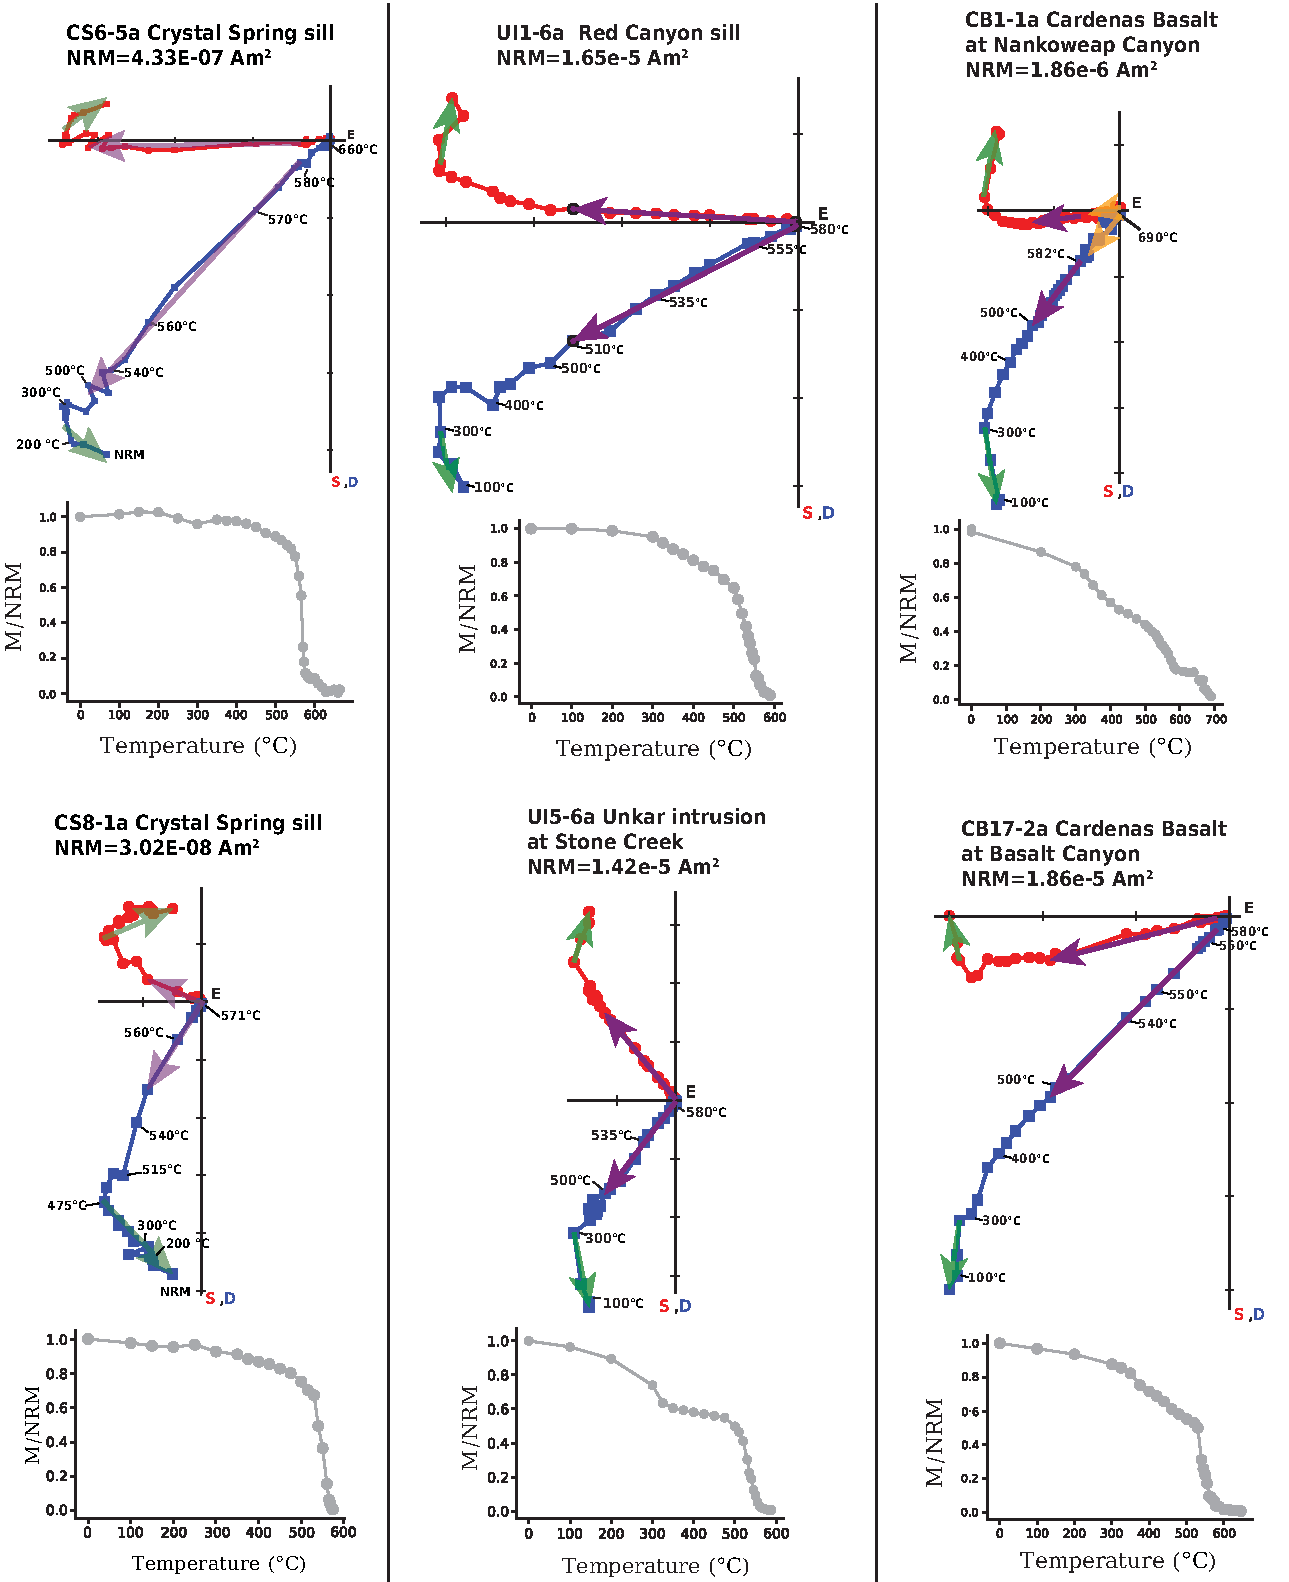
\includegraphics[width=0.78\textwidth]{figure/Zhang2024b/demag_plots.pdf}
\caption{\footnotesize Example orthogonal vector diagrams of specimen thermal demagnetization results from mafic sills that intruded the Crystal Spring Formation, mafic sills that intruded the Unkar Group, and the Cardenas Basalt. Total specimen magnetic moments (M) normalized by the natural remanent magnetizations (NRM) are plotted against temperature steps. The secondary overprint component (green) in the rocks can be removed by heating typically to $\sim$300\textdegree C, but can be up to $\sim$500\textdegree C, or efficiently removed by liquid nitrogen demagnetization. The interpreted primary component (purple) is origin-trending and typically unblocks sharply through $\sim$500-580\textdegree C. In some Cardenas lava flows such as CB1, a third component that unblocks up to $\sim$690\textdegree C exists, and is interpreted to be carried by hematite that formed during early oxidation. All orthogonal plots are shown in tilt-corrected coordinates.}
\label{fig:demag_plots}
\end{figure}

\subsection*{Intrusions in the Unkar Group and the Cardenas Basalt}
The two dated ca. 1098 Ma sills in eastern Grand Canyon (UI4 and UI5) and three intrusions near Hance Rapids and in Red Canyon (UI1, UI2, and UI3; Figure \ref{fig:geologic_maps}B) all yielded consistent within-site thermal demagnetization results and have similar thermal demagnetization behaviors between sites (Figure \ref{fig:demag_plots}, \ref{fig:equal_area_plots}). Typically, an origin-trending characteristic remanence component unblocks between 500\textdegree C and 585\textdegree C after a secondary overprint component that overlaps with the present local field direction is removed at lower temperatures (Figure \ref{fig:demag_plots}). This thermal demagnetization behavior indicates that the characteristic remanence components in these mafic intrusions are held by low-titanium titanomagnetite. Despite their similar demagnetization behaviors, the mafic intrusions record two distinct groups of remanence directions (Figure \ref{fig:equal_area_plots}). The ca. 1098 Ma mafic sills in Hotauta Canyon (UI4) and Stone Creek Canyon (UI5) record paleomagnetic directions to the northwest with steep inclinations, whereas the other three undated intrusions in eastern Grand Canyon have westerly directions and much shallower inclinations (Figure \ref{fig:demag_plots}, \ref{fig:equal_area_plots}). 

Thermal demagnetization of the 18 Cardenas Basalt lava flows yielded consistent site-level results (Figure \ref{fig:equal_area_plots}). After an overprint component that overlaps with the present local field direction was removed by heating up to 300\textdegree C (Figure \ref{fig:demag_plots}), the specimens typically demagnetized along an origin-trending path approaching the Curie temperature of magnetite. Some specimens continued to demagnetize up to the N\`eel temperature of hematite ($\sim$690\textdegree C; \cite{Ozdemir2006a}; Figure \ref{fig:demag_plots}). The unblocking temperature ranges indicate that (titano)magnetite and hematite are the dominant remanence-carrying minerals in the lava flows. Least-squares line fits made for the magnetite and hematite components have very similar directions in the same specimens (Figure \ref{fig:demag_plots}; CB1-1a). This result is consistent with the hematite having formed due to early oxidation of the lava flows indicating that it acquired remanent magnetization soon after the eruption of the lavas. 

\begin{figure}[h!]
\centering
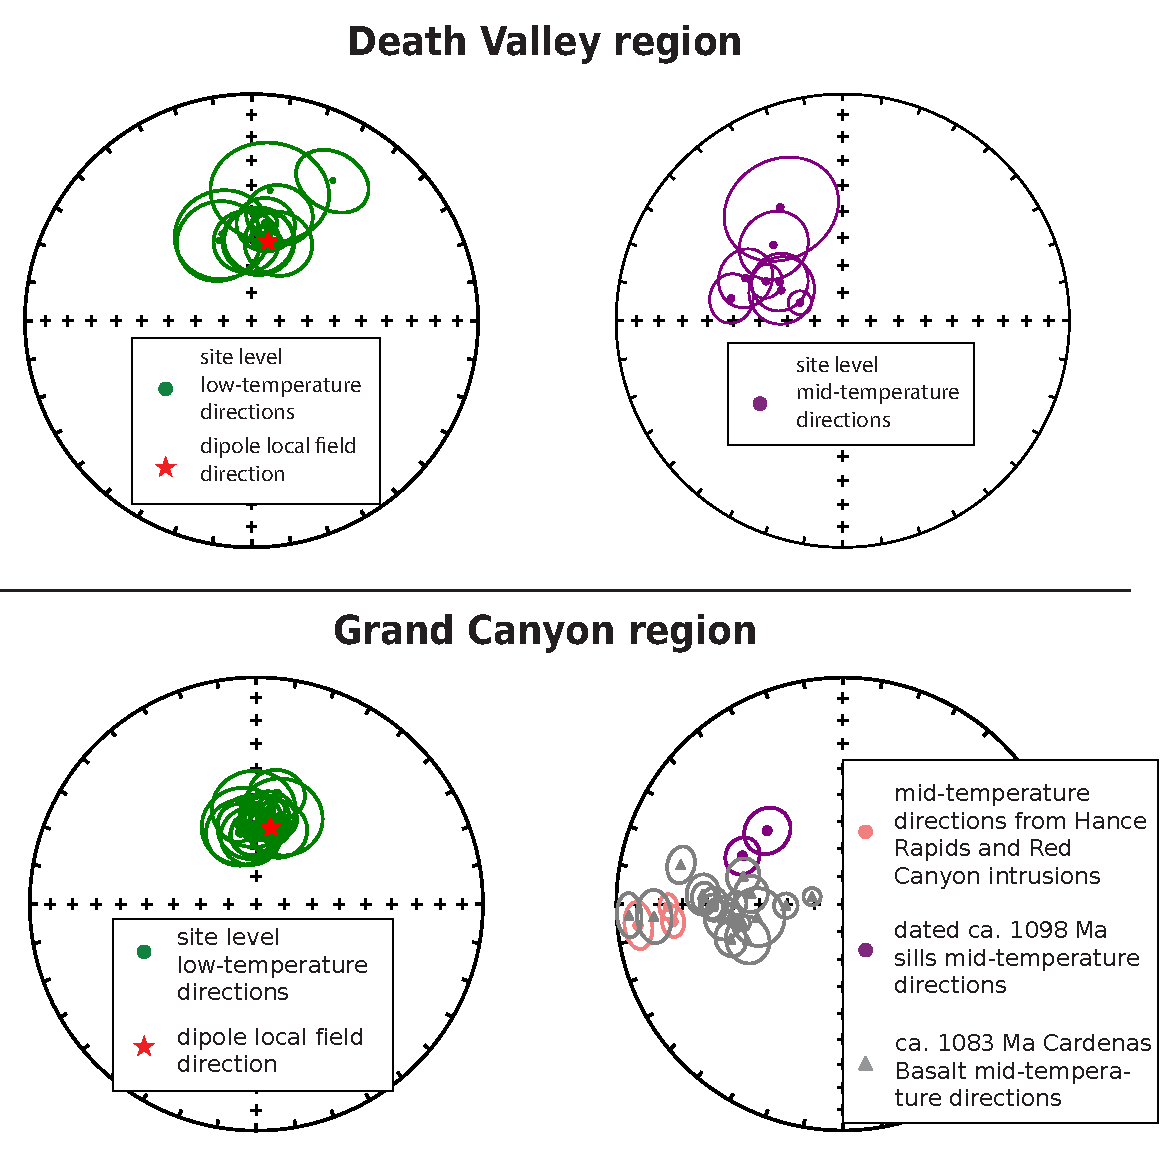
\includegraphics[width=0.8\textwidth]{figure/Zhang2024b/equal_area_plots.pdf}
\caption{\footnotesize Summary equal area diagrams for the site level directional results from the Death Valley region and the Grand Canyon region. The site level low-temperature components (green) in geographic coordinates are shown in context of present-day local field directions (red star) at the study localities. The mid-temperature directions (i.e. those that unblock over a temperature range consistent with magnetite) are shown in tilt-corrected coordinates. Note that the specimen directions from the mafic sills at Hotauta Canyon (UI4) and Stone Creek (UI5) (directions shown in purple) are more northerly and steeper than the specimen directions of Cardenas Basalt and the intrusions near Hance Rapids (shown in grey and pink).}
\label{fig:equal_area_plots}
\end{figure}

Site-level characteristic directions for all of the intrusions in Death Valley and Grand Canyon as well as Cardenas Basalt flows except for CB4 were calculated using the (titano)magnetite-bearing components. This component isolated through magnetite unblocking temperatures is referred to as the ``mid-temperature direction" in Figure \ref{fig:equal_area_plots}. For site CB4, all except for one specimen have antipodal components, both of which we interpret to be carried by hematite. The antipodal directions recorded within the same specimens may be the result of magnetic self-reversal associated with the oxidation of magnetite into maghemite which subsequently inverted into hematite \citep{Swanson-Hysell2011a}. A detailed description of the specimen results for site CB4 is presented in Figure S2. We combine the normal-polarity (i.e. directions pointing southwest and down) directions held by hematite in six samples together with a normal polarity direction carried by titanomagnetite in one sample for calculating a site mean direction for this flow. Seven samples collected from a baked interflow red sandstone layer (site CBS1) within 0.2 m of the base of lava flow CB11 yielded overlapping paleomagnetic directions with those from the overlying lava flow (Figure S3). We group the samples from the lava flow and the baked sediments as one site when calculating the mean direction and virtual geomagnetic pole (VGP). Figure \ref{fig:poles}B shows the VGPs of the two dated ca. 1098 Ma sills in eastern Grand Canyon (UI4 and UI5), VGPs of the the Cardenas Basalt sites, the mean pole position calculated for the Cardenas Basalt (pole longitude=183.9\textdegree, pole latitude=15.9\textdegree, N=18, A$^{95}$=7.4\textdegree, K=22.7; no rotation correction) and the VGPs of the intrusions near Hance Rapids and Red Canyon (UI1, UI2, and UI3). 

\section*{Discussion}

\subsection*{Timing of mafic magmatism in the SWLLIP}

Statistically indistinguishable high-precision U-Pb zircon ages from three sills in Death Valley, two sills in the Grand Canyon, and a sill in central Arizona were interpreted in \cite{Mohr2024a} to be consistent with decompression melting of an upwelling mantle plume ca. 1098 Ma. This hypothesis predicts that other thick sills in the region associated with the SWLLIP were also emplaced ca. 1098 Ma. Paleomagnetic directional data can provide another avenue to gain chronological insight on mafic units for which geochronology data have not been or cannot be developed. Rapid changes in Laurentia's pole position between ca. 1110 and 1070 Ma (Fig. \ref{fig:poles}D; \citep{Swanson-Hysell2019a}) enable such data to provide more informative temporal constraints than at many other time intervals.

The new paleomagnetic data from the dated sills in the Death Valley region and in the Grand Canyon are consistent with their high-precision U-Pb zircon ages. The 1097.91 $\pm$ 0.29 Ma CS1 sill  and the 1098.09 $\pm$ 0.91 Ma CS7 sill in Death Valley and the 1098.16 $\pm$ 0.59 Ma UI4 sill and 1098.09 $\pm$ 0.34 Ma UI5 sill in Grand Canyon have similar VGP positions at high latitudes in present-day coordinates (Figure \ref{fig:poles}A, B). The new paleomagnetic data further show that six additional undated sills in the Death Valley region have directions that are similar to those from the ca. 1098 Ma dated sills (Figs. \ref{fig:equal_area_plots} and \ref{fig:poles}). These data are consistent with all of the preserved Death Valley sills being associated with the ca. 1098 Ma pulse of mafic magmatism. Figure \ref{fig:poles}A shows the mean pole position calculated for all the Death Valley region sills. The pole overlaps within uncertainty with the pole position of the ca. 1096 Ma North Shore Volcanic Group upper southwest sequence of the Midcontinent Rift (Figure \ref{fig:poles}A; \cite{Swanson-Hysell2019a}). Although the paleomagnetic data of the Death Valley sills have directional uncertainties associated with potential vertical axis block rotations as detailed in the following section, these structural complexities do not take away the interpretation that the steep downward inclinations (Figure \ref{fig:demag_plots}) are compatible with a ca. 1098 Ma age. Additionally, the normal polarity of the magnetizations is consistent with the sills being emplaced during the earliest portion of the ca. 1099 to $<$1075 Ma Portage Lake normal polarity zone \citep{Swanson-Hysell2019a}---a late Mesoproterozoic superchron \citep{Driscoll2016b}. 

\begin{figure}[h!]
\centering
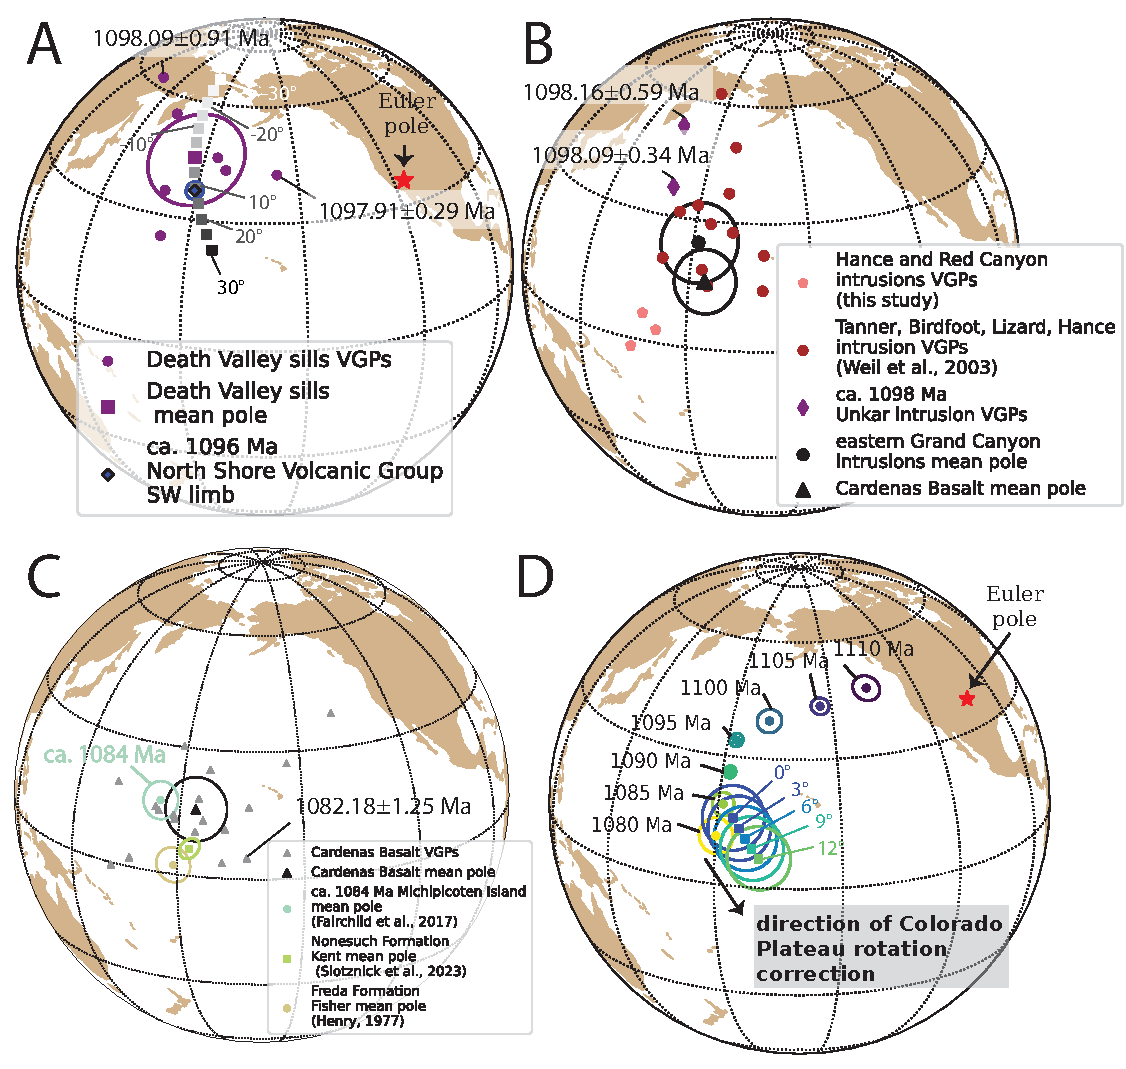
\includegraphics[width=0.8\textwidth]{figure/Zhang2024b/poles.pdf}
\caption{\footnotesize (A) Virtual geomagnetic poles (VGP) from the Death Valley mafic sills and the associated mean paleomagnetic pole plotted in context of the paleomagnetic pole position of the ca. 1096 Ma North Shore Volcanic Group southwest sequence pole from \cite{Swanson-Hysell2019a}. Variable vertical axis rotations of the mean Death Valley sills pole about an Euler pole located at 35.8\textdegree N, -116.4\textdegree E are shown. Positive (negative) values represent counterclockwise (clockwise) rotations about the Euler pole. (B) VGPs from the Cardenas Basalt and mafic sills within the Unkar Group are plotted together with the mean Cardenas Basalt pole and the mean pole calculated for intrusions that are hypothesized to be coeval with the Cardenas Basalt. VGPs of intrusions include those developed in this study as well as those from \cite{Weil2003a}. (C) The mean ca. 1082 Ma Cardenas Basalt paleomagnetic pole is plotted together with the ca. 1084 Ma Michipicotan Island Formation paleomagnetic pole \citep{Fairchild2017a} as well as the ca. 1075 Ma Nonesuch Formation pole \citep{Slotznick2023a} and lower Freda Formation pole \citep{Henry1977a}. (D) The Cardenas Basalt mean pole position is corrected for the hypothesized Colorado Plateau rotation with progressively larger rotations about an Euler pole position of -107\textdegree E, 37\textdegree N \citep{Bryan1990a}. The resultant pole positions are plotted in context of the synthesized Keweenawan Track (2 stage pole rotations and true polar wander scenario; \cite{Swanson-Hysell2019a}). Larger rotations result in less agreement between the Cardenas pole and the pole path based on Midcontinent Rift data. In plots (A) and (C) the VGPs from dated sills and the dated lava flow are labeled with their ages.}
\label{fig:poles}
\end{figure}   

The paleomagnetic pole position of the ca. 1082 Ma Cardenas Basalt plots at a lower latitude distinct from that of the ca. 1098 Ma mafic sills in Death Valley and the western Grand Canyon (Figure. \ref{fig:poles}A, C). Instead, the Cardenas Basalt pole is close to the paleomagnetic pole of the Michipicoten Island Formation of the Midcontinent Rift whose age is tightly bracketed to be between 1084.35 $\pm$ 0.20 Ma and 1083.52 $\pm$ 0.23 Ma \citep{Fairchild2017a}. In addition, the Cardenas Basalt pole is close to the ca. 1075 Ma paleomagnetic poles of the Nonesuch and Freda Formations \citep{Henry1977a, Slotznick2023a} of the Midcontinent Rift Oronto Group. That these localities $\sim$2,500 km apart yield overlapping pole positions when their poles are calculated under the assumption of a time-averaged dipolar field supports interpretations that the field was a stable dipole ca. 1080 Ma. Note that there is uncertainty in the Cardenas pole position associated with hypothesized rotation of the Colorado Plateau in the Mesozoic/Cenozoic (Fig. \ref{fig:poles}D; \cite[e.g.][]{Bryan1990a}). However, this uncertainty does not take away from the main conclusion as it does not affect interpretations of paleolatitude.

Overall, the large arc distance between the ca. 1098 Ma and the ca. 1082 Ma poles from southwestern Laurentia supports the interpretation based on Midcontinent Rift data that Laurentia experienced rapid plate motion from high latitudes toward the equator in the late Mesoproterozoic \citep{Davis1997a, Swanson-Hysell2009a}. This rapid motion is associated with the closure of the Unimos Ocean which culminating in the onset of Grenvillian collisional orogenesis \citep{Swanson-Hysell2023a}. 

\subsection*{Comparison to Mesoproterozoic paleomagnetic data from central Arizona}

Paleomagnetic data have been developed from mafic sills in central Arizona that intrude the Apache Group sedimentary rocks \citep{Helsley1972a, Harlan1993a, Donadini2011a}. Both \cite{Harlan1993a} and \cite{Donadini2011a} identified sills in the same region that record normal directions and reversed directions with the reversed directions having steeper inclinations. We compiled paleomagnetic data from these two studies with the goal of having each site be a distinct cooling unit. The resultant compilation is provided in Table S1. The individual site-level directions, corresponding virtual geomagnetic pole positions, and overall mean directions and poles are recalculated by polarity and plotted in Figure \ref{fig:Harlan_Donadini_compilation}. 

The compiled mean pole position of the normal-polarity mafic sills in central Arizona plots near the expected pole position of Laurentia ca. 1095 Ma based on data from the Midcontinent Rift rocks (Figure \ref{fig:Harlan_Donadini_compilation}; \cite{Swanson-Hysell2019a}). However, the distribution of the normal-polarity virtual geomagnetic pole positions is distinct from a Fisher distribution \citep{Fisher1953a}. Given that these VGPs show an elongate distribution along the Keweenawan Track (Figure \ref{fig:Harlan_Donadini_compilation}), we hypothesize that not all sills were emplaced during the same magmatic episode. However, that the sills have record a normal polarity and one sill yielded a U-Pb baddeleyite age of 1088 $\pm$ 11 Ma \citep{Bright2014a} which has an uncertainty that overlaps with an CA-ID-TIMS zircon U-Pb age of 1097.97 $\pm$ 0.12 Ma from a subhorizonal diabase sill in Salt River Canyon \citep{Mohr2024a} indicate that some of the sills could be coeval with the ca. 1098 Ma mafic sills in Death Valley and Grand Canyon. More precise radiometric dates that is paired with paleomagnetic data are needed from these sills. 

Despite the few records, the central Arizona sills with steep negative inclinations have a mean pole position distinct from that of the normal-polarity sills (Figure \ref{fig:Harlan_Donadini_compilation}). The mean pole plots near the older end of the Keweenawan Track, indicating a high paleolatitude for Laurentia at the time (Figure \ref{fig:Harlan_Donadini_compilation}). This configuration corresponds with the stable high-latitude position of Laurentia between ca. 1140 and 1105 Ma \citep{Ernst1993a, Piispa2018a, Swanson-Hysell2021c}. That reversed polarity is also consistent with the Alona Bay reversed polarity zone which has been identified during the onset of magmatism in the Midcontinent Rift \citep{Swanson-Hysell2019a}. The potential exists that in addition to there being a linkage between a SWLLIP plume that spread to the Midcontinent Rift ca. 1098 to 1096 Ma as hypothesized in \cite{Mohr2024a}, a plume upwelling under Laurentia at the onset of Midcontinent Rift development led to magmatism in both regions. To assess such temporal and dynamic connections, more precise ages of these reversed-polarity sills need to be determined. 

\begin{figure}[h!]
\centering
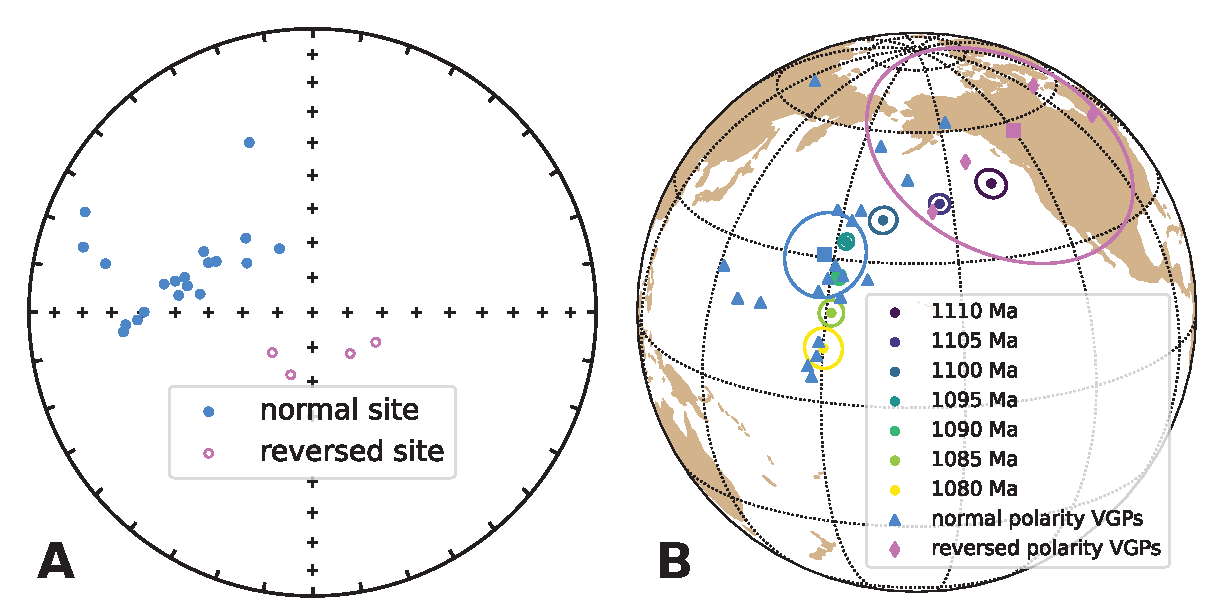
\includegraphics[width=0.8\textwidth]{figure/Zhang2024b/Harlan_Donadini_compilation.pdf}
\caption{(A) Compiled paleomagnetic directional data developed by \cite{Harlan1993a} and \cite{Donadini2011a} from mafic sills in central Arizona. The original data are selected with some recalculated such that each site included in this compilation is an individual cooling unit. Some sills record a reversed polarity with steep inclinations (orchid), while the other sills record a normal polarity with shallower inclinations (blue). The compiled data are in Table S1. (B) Virtual geomagnetic poles (VGP) of individual cooling units and mean paleomagnetic poles of the central Arizona mafic sills are plotted in context of the synthesized Keweenawan Track of \cite{Swanson-Hysell2019a} (two stage pole with true polar wander scenario). The mean pole position of sills with reversed polarity is close to the older end of the Keweenawan Track while the mean normal-polarity pole plots close to the expected pole position ca. 1095 Ma.}
\label{fig:Harlan_Donadini_compilation}
\end{figure}

\subsection*{Death Valley region sills}
\subsubsection*{Structural complexity associated with Neogene extension}

The Death Valley region experienced complex deformation associated with extension and shearing during Neogene extensional tectonism \cite[e.g.][]{Wernicke1988a}. It has been suggested that tilting associated with generally west-dipping normal faults, as well as vertical axis rotations of crustal blocks associated with conjugate strike-slip fault systems principally accommodated the deformation \cite[e.g.][]{Serpa1996a}. Geologic mapping and associated structural analyses suggest that strike-slip faults are coeval with normal faulting and have a left-lateral sense when they strike eastward or northeastward (e.g., Garlock fault; Figure \ref{fig:geologic_maps}A) and a right-lateral sense when they strike northwestward (e.g., south Death Valley fault;  Figure \ref{fig:geologic_maps}A); \cite{Wright1976a, Serpa1996a, Pavlis2014a}). However, the extent to which extension is partitioned between the normal faulting and strike-slip faulting have long been debated \cite[e.g.][]{Burchfiel1965a, Guth1981a, Snow1989a, Holm1993a, Petronis2002a, Renik2013a}. 

The Death Valley region mafic sills that we sampled belong to different range-scale crustal blocks, including the Panamint Mountains, the Black Mountains, and the Nopah Range (Figure \ref{fig:geologic_maps}A). Sedimentary strata in the Crystal Spring Formation in these ranges dip variably to the east (Figure \ref{fig:geologic_maps}A). The mafic sills intruded parallel to the bedding of the Crystal Spring Formation, often taking advantage of contacts between different lithologies such as the contact between the argillite facies and the cherty dolomite facies. The dips of the sills vary between $\sim$23\textdegree to $\sim$86\textdegree. The paleomagnetic directions for the sills are much better grouped when corrected for this tilt (dec=302.8\textdegree, inc=58.0\textdegree, n=8, a$_{95}$=9.5\textdegree, k=34.8) than when considered in geographic coordinates without tilt correction (dec=295.1\textdegree, inc=8.9\textdegree, a$_{95}$=21.6\textdegree, k=7.5) (Figure S4). This result is consistent with the interpretation that the characteristic remanence component carried by (titano)magnetite in the sills is a primary remanence acquired during initial cooling prior to tilting of the Crystal Spring Formation. 

It is more challenging to correct for vertical axis rotations in the Death Valley region as the degrees of rotations are poorly constrained. Sills CS1, CS2, and CS6 are from Warm Spring Canyon of the Panamint Mountains, which is an east-tilting block now bounded by the right-lateral Panamint Valley fault to the west and the left-lateral Garlock fault to the south (Figure \ref{fig:geologic_maps}; \cite{Snow1989a, Snow2000a}). \cite{Stewart1983a} interpreted that the Panamint Range was detached from above the crystalline core of the Black Mountains and translated some 80 km northwest along west dipping low-angle detachment faults. \cite{Petronis2002a} developed paleomagnetic data from Miocene intrusive rocks in the central Panamint Range and Miocene volcanic rocks in the eastern part of the range. Their data from the central range show a pole position that overlaps with that expected for no rotation, which they interpreted to indicate minimal amount of vertical axis rotation. They did find a discordance between paleomagnetic declinations developed from Miocene volcanic rocks in the eastern Panamint Range which appear to show substantial clockwise vertical axis rotations since the Miocene (27.6\textdegree $\pm$ 15.2\textdegree, calculated based on nine paleomagnetic sites). However, \cite{Petronis2002a} cautioned against interpreting there to have been a large vertical axis rotation in the eastern range as their data may undersample paleosecular variation. In the northwest Black Mountains, paleomagnetic data developed from Miocene intrusive rocks and Proterozoic basement rocks have been interpreted to indicate large vertical axis rotations as a result of oroclinal bending associated with right-lateral shear along the Death Valley fault zone (up to $\sim$80\textdegree; \cite{Holm1993a}). However, paleomagnetic data developed from late Miocene igneous rocks in the eastern Panamint Mountains indicate minimal rotations in the region \citep{Petronis2002a}. These data led \cite{Petronis2002a} to hypothesize that the significant vertical axis rotation observed by \cite{Holm1993a} could be restricted to the western range where the basement block is sheared along the Death Valley fault zone (Figure \ref{fig:geologic_maps}). In this case, the more southeastern parts of the Black Mountains fault block, where sills CS7, CS8, and CS9 were collected, and distal from the fault zone, may have experienced relatively insignificant vertical axis rotation (Figure \ref{fig:geologic_maps}). In the Nopah Range, where site CS13 was sampled within the crystalline basement (Figure \ref{fig:geologic_maps}), no quantitative constraints exist on the amount of vertical axis rotation. Models that involve no rotation to those with up to 30\textdegree\ of clockwise rotation since the Neogene have all been proposed and interpreted to broadly fit the structural evidence in the region \cite[e.g.][]{Serpa1996a, Pavlis2014a}. Rotation in the Alexander Hills (site CS12) is similarly poorly constrained. 

The limited number of paleomagnetic sites from mafic sills in the different range blocks preclude the assessment of vertical axis rotation at each sampling locality (Figure \ref{fig:geologic_maps}A). This limitation is due to the secular variation of the geomagnetic field, which makes it such that single VGPs or low numbers of VGPs do not give accurate or precise estimate of the mean paleomagnetic pole position to be compared to a reference path. However, the tilt-corrected VGPs from the eight mafic sills with well-resolved magnetizations can provide insights into the structural history of the study region when viewed in context of Laurentia's apparent polar wander path in the late Mesoproterozoic. The tilt-corrected virtual geomagnetic poles from all sills are grouped at northern high latitudes, and the mean pole position plots close to the inverted pole position for ca. 1100 Ma and 1095 Ma (Figure \ref{fig:poles}A; \cite{Swanson-Hysell2019a}). This position is consistent with the ca. 1098 Ma age given by the indistinguishable zircon U-Pb ages from the three dated sills (Figure \ref{fig:SWLLIP_overview}B; \cite{Mohr2024a}). The overlapping pole positions between the Death Valley sills mean pole and poles from rocks of similar age in the Midcontinent Rift of the continental interior indicate that any vertical axis rotations were not large enough to have displaced the pole from the path ($<$30\textdegree\ ; Figure \ref{fig:poles}A).

Until more detailed and quantitative spatial and temporal constraints are developed for the different range blocks of the Death Valley region, it remains inconclusive as to the amount of Neogene vertical axis rotation correction to apply to these Mesoproterozoic sill directions. Given these vertical axis rotation uncertainties, we believe it is the best to not include the Death Valley mafic sills paleomagnetic pole into curated paleogeography databases. Nevertheless, the pole with no vertical axis rotations to the sites is consistent with the expected ca. 1098 position of Laurentia.

\subsection*{Grand Canyon region intrusions and Cardenas Basalt}

\cite{Weil2003a} developed paleomagnetic data from 13 mafic intrusions (in the eastern Grand Canyon between RM68 and RM78; Fig. \ref{fig:geologic_maps}) as well as three Cardenas Basalt flows at Basalt Canyon. Using the framework that the intrusions were time-equivalent with one another and with the lavas, \cite{Weil2003a} grouped all paleomagnetic directions from the intrusive and extrusive rocks to calculate a mean paleomagnetic pole position. There is an overall consistency in the directions of those studied units which is consistent with this interpretation. The pole was assigned an age of 1090.6 $\pm$ 4.5 Ma based on an $^{40}$Ar/$^{39}$Ar age developed from biotite collected within Unkar sedimentary rocks baked by a sill in the western Grand Canyon at RM131 (outside their paleomagnetic study region; \cite{Weil2003a}). This mean pole position has been included in pole compilations \cite[e.g.][]{Evans2021a} and used to constrain Laurentia's apparent polar wander path in the late Mesoproterozoic. 

The recent high-precision zircon U-Pb ages from the two sills in western Grand Canyon and the thick Cardenas Basalt flow at Nankoweap Canyon indicate that some of the sills in the Unkar Group are not feeders to the Cardenas Basalt given that their ca. 1098 Ma ages are $\sim$16 Myr older than the lavas which erupted ca. 1082 Ma (Figure \ref{fig:SWLLIP_overview}B; \cite{Mohr2024a}). Improvements in the paleomagnetic and geochronological records from the Midcontinent Rift \cite[e.g.][]{Tauxe2009a, Kulakov2013b, Fairchild2017a, Swanson-Hysell2019a} and advances in synthesizing apparent polar wander paths that incorporate both positional and temporal uncertainty, have led to the development of an updated ca. 1110 and 1070 Ma Keweenawan Track pole path (Figure \ref{fig:poles}; \cite{Swanson-Hysell2019a, Rose2022a}). In context of this updated pole path, the new geochronology data from \cite{Mohr2024a} would predict that the ca. 1098 sills and the ca. 1082 Ma Cardenas Basalt would have recorded distinct pole positions with a large ($\sim$23\textdegree) angular distance between them \citep{Swanson-Hysell2019a, Rose2022a}. 

The new paleomagnetic data from the Grand Canyon are consistent with the updated geochronology. Although there are not enough dated ca. 1098 Ma mafic sills from the Grand Canyon that paleosecular variation can be averaged out and a mean paleomagnetic pole position can be calculated, the VGPs from the two dated mafic sills both plot at high latitudes, close to the ca. 1100 Ma pole path position based on Midcontinent Rift data (Figure \ref{fig:poles}). On the other hand, the VGPs of the 18 Cardenas Basalt lava flows are consistent with being Fisher distributed (Figure S5), with a mean pole position at a low latitude. This pole position overlaps with Laurentia's pole path at ca. 1085 Ma and ca. 1080 Ma (Figure \ref{fig:poles}B). 

Despite a lack of direct field evidence for feeder dikes, and that the two dated sills in western Grand Canyon cannot be feeders to the lava flows given their older age (Figure \ref{fig:SWLLIP_overview}, \ref{fig:geologic_maps}B), there would have been feeder dikes to the Cardenas Basalt that crosscut older Unkar sedimentary rocks. While high-precision geochronology on individual intrusions would be needed to unambiguously distinguish potential Cardenas feeders from older intrusions, paleomagnetic data have the potential to provide insight given the rapid apparent polar wander of Laurentia at the time. The VGPs of the Hance sill (UI3), Hance dike (UI2), and the Red Canyon sill (UI1) are well-grouped at equatorial latitudes (Figure \ref{fig:poles}B). These poles are close to the inverted ca. 1080 Ma pole position of the Keweenawan Track. Geographically, these intrusions are close to the Cardenas Basalt near Basalt Canyon and far from the dated ca. 1098 Ma sills (Fig. \ref{fig:geologic_maps}B). Geochemical data developed by \cite{Larson1994a} also show that the Hance sill and Cardenas Basalt have similar rare earth element patterns (Figure S6). These data are consistent with the interpretation of the Hance intrusions (UI1, UI2, and UI3) as feeders to the Cardenas Basalt. The Birdfoot dikes, Lizard dikes, and Tanner dikes studied by \cite{Weil2003a} are also close to Basalt Canyon (Fig. \ref{fig:geologic_maps}). A mean paleomagnetic pole based on VGPs from these intrusions (i.e. dike data from \cite{Weil2003a}) and from the Hance intrusions of this study is calculated and shown in Figure \ref{fig:poles}B. This pole position is similar to that from the Cardenas Basalt. The VGPs from these eastern Grand Canyon intrusions pass a common mean test with the Cardenas Basalts VGPs (Fig. \ref{fig:poles}). While some of the individual VGPs plot at higher latitudes which could be consistent
with the ca. 1098 Ma pulse of magmatism, the overall similarity of directions is consistent with interpretation of some of these eastern Grand Canyon intrusions being ca. 1082 Ma feeders to the Cardenas Basalt. In contrast, the geochronology and paleomagnetic directions of the western sills show them to be associated with the older ca. 1098 Ma magmatism. 

\subsubsection*{Complexity associated with hypothesized Colorado Plateau rotation}

The Grand Canyon is located at the southwestern edge of the Colorado Plateau which was uplifted, folded, and tilted as a result of compression associated with the subduction of the Farallon plate underneath the North American plate during the late Cretaceous to Paleogene Laramide orogeny \citep{Yonkee2015a, Karlstrom2012a, Timmons2012a, Karlstrom2022a}. Structural analyses have suggested that the plateau rotated clockwise as a rigid block with respect to cratonic North America due to shear during the orogeny \cite[e.g.][]{Hamilton1981a, Hamilton1988a}. Efforts to quantitatively constrain the amount of rotation using paleomagnetic data have given different results albeit with agreement that the sense of rotation is clockwise. \cite{Kent1993a} and \cite{Steiner2003a} took the approach of developing Mesozoic paleomagnetic poles from the Colorado Plateau and comparing them with reference poles developed from cratonic North America to estimate the amount of rotation. Those studies gave relatively large estimates of interpreted rotations of 13.5 $\pm$ 3.5\textdegree and 9.0 $\pm$ 3.3\textdegree, respectively. Challenges exist with the approach of estimating the amount of rotation based on single paleomagnetic pole positions such as issues with age uncertainty between poles and reference pole positions. \cite{Garza1998a} and \cite{Bryan1990a} used approaches based on comparing multiple paleomagnetic poles through the Paleozoic to Mesozoic from on and off the plateau simultaneously and interpreted that the amount of rotation is $\sim$5\textdegree. These smaller estimated rotations are more consistent with the structural evidence of a small magnitude of strike-slip translation along the boundary of the Colorado Plateau \cite[e.g.][]{Woodward1997a}. 

The Cardenas Basalt paleomagnetic pole presents an opportunity of using Mesoproterozoic data to gain insights into Colorado Plateau rotation. Figure \ref{fig:poles}D shows the paleomagnetic pole of the Cardenas Basalt in context of the synthesized Keweenawan Track (two Euler scenario; \cite{Swanson-Hysell2019a}). As a progressively larger correction for Colorado Plateau rotation (using an Euler pole at -107\textdegree E, 37\textdegree N; \cite{Bryan1990a}) is applied, the Cardenas Basalt pole moves farther away from the Keweenawan Track and no longer overlaps with the inverted pole positions at ca. 1080 Ma after a 6\textdegree correction (Figure \ref{fig:poles}D). While this result is consistent with the interpretation that the Colorado Plateau experienced a relatively small amount of rotation ($<$6\textdegree\ ), it not feasible to use a single Cardenas Basalt pole to constrain the amount of Colorado Plateau rotation more precisely than previous estimates, as the Fisher 95\% angular uncertainty associated with the pole position itself is 11.8\textdegree\ (Figure \ref{fig:poles}). Future efforts to constrain Colorado Plateau rotation can incorporate both Mesoproterozoic and Mesozoic poles.

\subsection*{Outlook for future work in the southwestern Laurentia}

The high-precision geochronology data developed by \cite{Mohr2024a} revise the southwestern Laurentia large igneous province to feature the emplacement of ca. 1098 Ma thick mafic intrusions (often $>$100 m in thickness; \cite{Wright1967a}) from eastern California to central Arizona. The indistinguishable ages from these thick mafic intrusions across a large areal extent reveal the voluminous and rapid nature of emplacement of the magmatic pulse of the SWLLIP. This large igneous province could include more undated mafic intrusions that could be constrained with paleomagnetic data. \cite{Bright2014a} suggested that some mafic sills in New Mexico could also be a part of the SWLLIP, but the available geochronology data does not have the resolution to robustly test the hypothesis. In Figure \ref{fig:SWLLIP_overview}, we present an updated version of the areal extent of the SWLLIP as being defined by the ca. 1098 Ma geochronologically constrained mafic magmatism. 

Both geochronology and paleomagnetic data indicate that the Cardenas Basalt in the Grand Canyon was emplaced during a distinct episode of magmatism younger than the SWLLIP mafic sills. However, whether the emplacement of the lava flows is associated with a localized regional event or another period of large igneous province style magmatism remains to be tested. One mafic sill in the Dead Mountains of eastern California yielded a weighted mean zircon U-Pb age of 1082.60 $\pm$ 0.30 \cite{Mohr2024a}, which is indistinguishable with the 1082.18 $\pm$ 1.25 Ma age of the Cardenas Basalt (Figure \ref{fig:SWLLIP_overview}B). These ages indicate that the ca. 1082 Ma mafic magmatism could have stretched over at least 300 km. Over how large of a region did this ca. 1082 Ma magmatism occur?

The paleomagnetic pole of the Cardenas Basalt can help further constrain the Keweenawan Track given that it is younger than any pole developed from Midcontinent Rift volcanics. Currently, the younger end of the Keweenawan Track is constrained by the ca. 1084 Ma lava flows of the Michipicoten Island Formation and the ca. 1080-1050 Ma Nonesuch Formation and Freda Formation of the Oronto Group \citep{Swanson-Hysell2019a}. Uncertainties associated with correcting for inclination shallowing in sedimentary records and constraining the age of detrital remanence magnetization have led to the post-1085 Ma portion of the path to be less constrained than that from ca. 1110 to 1085 (Figure \ref{fig:poles}). The new temporally constrained Cardenas Basalt pole adds a valuable new constraint to Laurentia's database of paleomagnetic poles given as it is younger than the Michipicoten Island Formation. Additionally, as a pole from volcanics no correction for inclination shallowing is necessary. Once the amount of Colorado Plateau rotation and the associated uncertainty is better constrained, an updated Keweenawan Track can be developed using the new site-based resampling approach of \cite{Gallo2023a}. This method has the machinery to incorporate uncertainties in pole position, geochronology, as well as the magnitude of Colorado Plateau rotation correction into a synthesized path.

\section{Acknowledgments}
Project research was funded by NSF CAREER grant EAR-1847277 to N.L.S.-H. Additional research support came from an H2H8 research grant to Y.Z. as well as a UC Berkeley summer undergraduate research fellowship and a UC Berkeley Department of Earth Science Ramsden grant to N.A. We thank participants in the 2021 Grand Canyon Supergroup field forum for stimulating interactions in the canyon. National Park Service Permits for sampling within Grand Canyon National Park and Death Valley National Park are gratefully acknowledged.

%\nocite{Fisher1987a, Tauxe1991a, McFadden1990a, Haggerty1967a, Hedley1968a, McClelland1987a, McClelland1993a, Swanson-Hysell2011a, Driscoll2016b, Heslop2023a}
